\def\pgfsysdriver{pgfsys-dvipdfm.def}
%\documentclass[aspectratio=1610]{beamer}
\documentclass{beamer}
\usetheme[progressbar=head, titleformat=allcaps,block=fill]{metropolis}
\usepackage[orientation=landscape,size=custom,width=16,height=11.15,scale=.5,debug]{beamerposter}

%%% PACKAGES AND INPUTS
\usepackage{pgfopts}
\usepackage{pgfpages}
\usepackage{graphicx}
\usepackage{xcolor}
\usepackage{tikz}
\usetikzlibrary{3d,hyperref}
\usepackage{verbatim}
\usepackage{comment}
%\input{153controls}
\usepackage{pgfplots}
\usepackage{linalgjh}

\usepackage{multicol}


%%% POLAR SETUP
\usepgfplotslibrary{polar}
\pgfplotsset{compat=1.10}
\pgfplotsset{mypolarplot/.style={%
  clip=false, % needed for double line (last \addplot command)
  domain=0:360, % plot full cycle
  samples=180, % number of samples; can be locally adjusted
  grid=both, % display major and minor grids
  major grid style={black}, 
  minor x tick num=3, % 3 minor x ticks between majors
  minor y tick num=1, % 1 minor y tick between majors
  xtick={0,45,...,359},
  xticklabels={%
    $0$,
    $\frac{ \pi}{4}$,
    $\frac{ \pi}{2}$,
    $\frac{3\pi}{4}$,
    $\pi$,
    $\frac{5\pi}{4}$,
    $\frac{3\pi}{2}$,
    $\frac{7\pi}{4}$
  },
  yticklabel style={anchor=north}, % move label position
}}

%%%% COLORS
\definecolor{gold}{HTML}{ffb81c}
\definecolor{heypurple}{HTML}{6B0FFF}
\definecolor{darkgold}{HTML}{5A440D}
\definecolor{darkblue}{HTML}{00268D}
\definecolor{proof}{RGB}{55,54,172}
\definecolor{nicegreen}{RGB}{0,127,35}
\definecolor{remgrey}{RGB}{179,179,179}
\definecolor{Purple}{HTML}{3C0940}
\definecolor{darkgreen}{HTML}{214009}
\definecolor{Orange}{HTML}{7F2000}
\definecolor{Blue}{HTML}{003E78}
\definecolor{Gold}{HTML}{FFCB0A}
\definecolor{gvsublue1}{HTML}{0065a4}
\definecolor{gvsublue2}{HTML}{88B3DA}
\definecolor{unlred}{HTML}{D00000}
\definecolor{DordtGrey}{RGB}{127,127,127}
\definecolor{newred}{HTML}{85140D}
\definecolor{msugreen}{HTML}{023328}
\definecolor{seafoam}{HTML}{127F67}
\definecolor{mnmaroon}{HTML}{790018}
\definecolor{mngold}{HTML}{FFD75F}
\definecolor{fallfoliage}{HTML}{763626}
\definecolor{stone}{HTML}{336B87}
\definecolor{shadow}{HTML}{2A3132}
\definecolor{grass}{HTML}{486B00}
\definecolor{thundercloud}{HTML}{505160}
\definecolor{meadow}{HTML}{598234}
\definecolor{ink}{HTML}{20232A}
\definecolor{rubyred}{HTML}{A01D26}
\definecolor{stormysea}{HTML}{335252}
\definecolor{rust}{HTML}{AA4B41}
\definecolor{forest}{HTML}{1E434C}
\definecolor{crimson}{HTML}{8D230F}
\definecolor{vtgold}{HTML}{C99E10}
\definecolor{vtrust}{HTML}{9B4F0F}

%%%% BEAMER THEMES AND OPTIONS
%\usetheme[progressbar=head,block=fill]{metropolis}
%\setbeameroption{show notes on second screen}
%\metroset{titleformat=smallcaps,block=transparent}
%\usecolortheme{owl}
\setbeamercolor{progress bar}{fg=heypurple,bg=heypurple!30}
\setsansfont[BoldFont={Graphik Semibold},Numbers={Produkt}]{Graphik}


%%% Dordt
%\setbeamercolor{alerted text}{fg=gold}
%\setbeamercolor{normal text}{fg=black}
%%%\setbeamercolor{block}{transparent}
%%%\setbeamercolor{sectionpage}{bg=white}
%%%\setbeamercolor{titleformatpage}{bg=white}
%\setbeamercolor{frametitle}{fg=gold,bg=black!2}
%%%%% GREEN OPTION
%%%\setbeamercolor{alerted text}{fg=seafoam} 
%%%\setbeamercolor{frametitle}{bg=msugreen}



%%% Purple
\setbeamercolor{alerted text}{fg=heypurple}
\setbeamercolor{normal text}{fg=black}
%%\setbeamercolor{block}{transparent}
%%\setbeamercolor{sectionpage}{bg=white}
%%\setbeamercolor{titleformatpage}{bg=white}
\setbeamercolor{frametitle}{fg=heypurple,bg=black!2}
%%%% GREEN OPTION
%%\setbeamercolor{alerted text}{fg=seafoam} 
%%\setbeamercolor{frametitle}{bg=msugreen}

%%% MN OPTION
%\setbeamercolor{alerted text}{fg=gold}
%\setbeamercolor{frametitle}{bg=mnmaroon}

%%% FALL MOUNTAIN
%\setbeamercolor{alerted text}{fg=fallfoliage}
%\setbeamercolor{frametitle}{bg=shadow}
%\setbeamercolor{alerted text}{fg=stone}
%\setbeamercolor{alerted text}{fg=grass}

%%% ICELAND
%\setbeamercolor{alerted text}{fg=meadow}
%\setbeamercolor{frametitle}{bg=thundercloud}


%%% VERMONT
%\setbeamercolor{alerted text}{fg=crimson}
%\setbeamercolor{alerted text}{fg=vtrust}
%\setbeamercolor{frametitle}{bg=thundercloud}


%%% INDUSTRIAL
%\setbeamercolor{alerted text}{fg=rubyred}
%\setbeamercolor{frametitle}{bg=ink}

%%% SAN FRANCISCO
%\setbeamercolor{alerted text}{fg=rust}
%\setbeamercolor{frametitle}{bg=stormysea}


%%%% MACROS
\def\rem#1{{\hfill \textit{\tiny {\color{remgrey} {#1}}}}}
\def\h#1{\alert{#1}}
\def\C{{\mathbb C}}
\def\Z{{\mathbb Z}}
\def\F{{\mathbb F}}
\def\bF{{\mathbb F}}
\def\Q{{\mathbb Q}}
\def\R{{\mathbb R}}
\def\P{{\mathbb P}}
\def\A{{\mathbb A}}
\def\N{{\mathbb N}}
\def\i{\mathbf i}}
\def\j{\mathbf j}}
\def\k{\mathbf k}}
\def\proj{{\text{proj}}}
\def\comp{{\text{comp}}}
\def\set#1{\left\{ {#1} \right\}}
\def\setof#1#2{{\left\{#1\,:\,#2\right\}}}


%%%% ENVIRONMENTS
\newenvironment{proof-idea}{\noindent{\alert{Proof Idea.}}\hspace*{1em}}{\qed\bigskip\\}
\newtheorem{conj}{Conjecture}
\newtheorem{prop}{Proposition}
\newtheorem{cor}{Corollary}
\newtheorem{defn}{Definition}
\newtheorem{question}{Question}
\newtheorem{goal}{Goal}

\usepackage{cancel}
\newcommand\lheq{\mathrel{\overset{\makebox[0pt]{\mbox{\normalfont\tiny\sffamily \alert{L'H}}}}{=}}}

\title{\S 3.1: Using Derivatives to Identify Extreme Values}
%\subtitle{Welcome!}
\author{Dr.\ Mike Janssen}
\date{March 12, 2021}

\begin{document}




\frame{\titlepage}





\frame{
	\frametitle{Announcements}
	
	\begin{itemize}
	\item 
	
	
\end{itemize}

}






\frame{
	\frametitle{Recall: Critical Numbers and FDT}
	
	\begin{definition}
We say that a function $f$ has a critical number at $x=c$ provided that
\begin{enumerate}
	\item $c$ is in the domain of $f$, and
	\item $f'(c)=0$ OR $f'(c)$ is undefined.
\end{enumerate}
\end{definition}

\pause

\begin{theorem}[First Derivative Test]
If $p$ is a critical number of a continuous function $f$ that is differentiable near $p$ (except possibly at $x=p$), then $f$ has a relative maximum at $p$ if and only if $f'$ changes sign from positive to negative at $p$, and $f$ has relative minimum at $p$ if and only if $f'$ changes sign from negative to positive at $p$.
\end{theorem}

}


\frame{
	\frametitle{Activity 3.1.2}

}


\frame{
	\frametitle{Second Derivatives}
	
	\begin{center}
		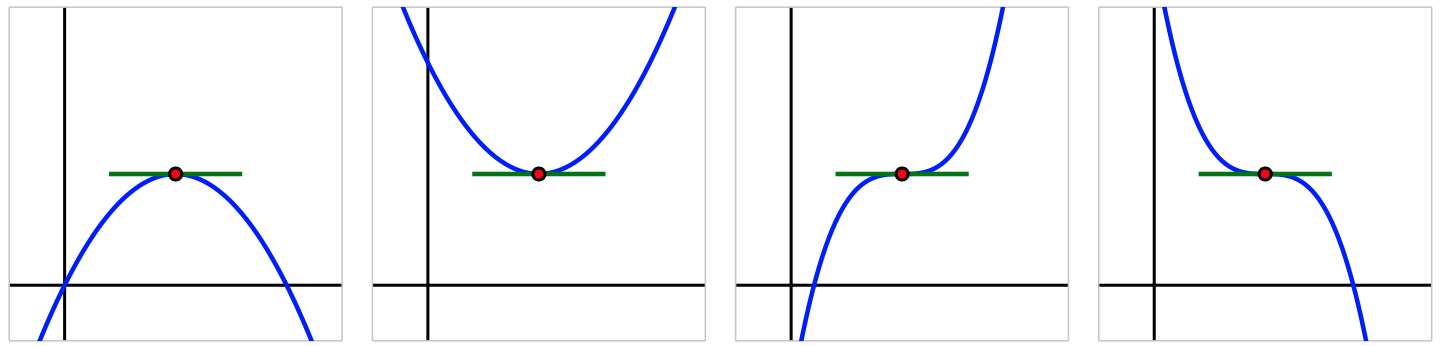
\includegraphics[width=5in]{img/2dtest.png}
	\end{center}
	
	\pause
	
	\begin{theorem}[Second Derivative Test]
	
	If $p$ is a critical number of a continuous function $f$ such that $f'(p) = 0$ and $f''(p)\ne 0$, then $f$ has a relative maximum at $p$ if $f''(p) < 0$, and $f$ has a relative minimum at $p$ if $f''(p) > 0$.
		
	\end{theorem}
	
	}
	
	
	\frame{
		\frametitle{Points of inflection}
		
		\begin{definition}
		
			If $p$ is a value in the domain of a continuous function $f$ at which $f$ changes concavity, then we say that $(p, f(p))$ is an \textbf{inflection point} of $f$.
		
		\end{definition}
	
		
		\pause
		
		\alert{Question:} What is required for a function to \emph{change} concavity?
	
	}


\frame{
	\frametitle{Activities 3.1.3-3.1.4}
}

\section{\S 3.2: Using Derivatives to Describe Families of Functions}

\frame{
	\frametitle{Preview Activity Discussion}
	
	\pause
	
	\alert{Goal:} Examine \emph{families} of functions in terms of certain \emph{parameters}, certain constants that repeatedly appear in applications of a given function.
}


\frame{
	\frametitle{Example}
	
	Consider the function
	\[
		f(x) = a\sin(bx), \ \ a, b\ne 0
	\]
	on the interval $[0, 2\pi]$.
	Let's:
	\begin{itemize}
	\item find the critical numbers of $f$ and construct a first derivative sign chart, taking into account the possible signs of $a$ and $b$
	\item Find $p''$ and construct a second derivative sign chart
	\item Sketch and label typical graphs of $f$
\end{itemize}

}

\frame{
	\frametitle{Activity 3.2.2-3.2.4}

}






\end{document}